\section{42 - MAT - FA 5.1, FA 5.3, FA 2.2, AN 1.3, FA 1.5 - CO$_2$-Gehalt der Atmosphäre - Matura 2013/14 2. Nebentermin}

\begin{langesbeispiel} \item[0] %PUNKTE DES BEISPIELS
				 Die Atmosphäre besteht zu ca. 78\,\% aus Stickstoff und zu ca. 21\,\% aus Sauerstoff. Kohlendioxid (CO$_2$) ist nur in Spuren vorhanden. Dennoch ist CO$_2$ zusammen mit Wasserdampf der Hauptverursacher des natürlichen Treibhauseffektes. Seit 250 Jahren ist der CO$_2$-Gehalt der Atmosphäre massiv gestiegen (siehe Abb. 1). Man vermutet, dass dadurch der Treibhauseffekt verstärkt wird.

	\begin{center}
	\resizebox{0.6\linewidth}{!}{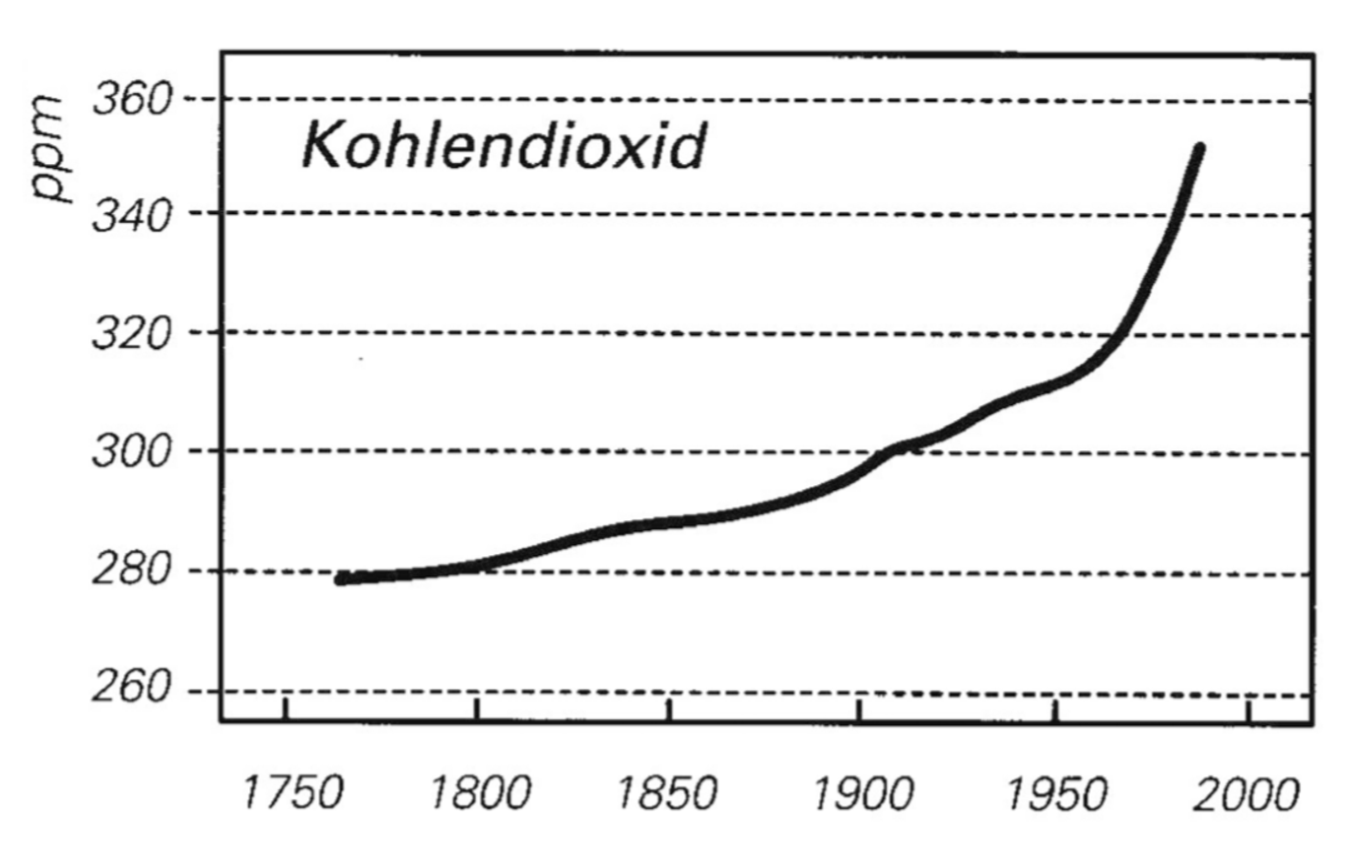
\includegraphics{../Bilder/Bild42-1.eps}}
	\end{center}
	\begin{footnotesize}\textit{Abb. 1: Aufzeichnung der mittleren CO$_2$-Konzentration in der Atmosphäre von 1760 bis 1980}\end{footnotesize}
	
	\begin{center}
	\resizebox{0.6\linewidth}{!}{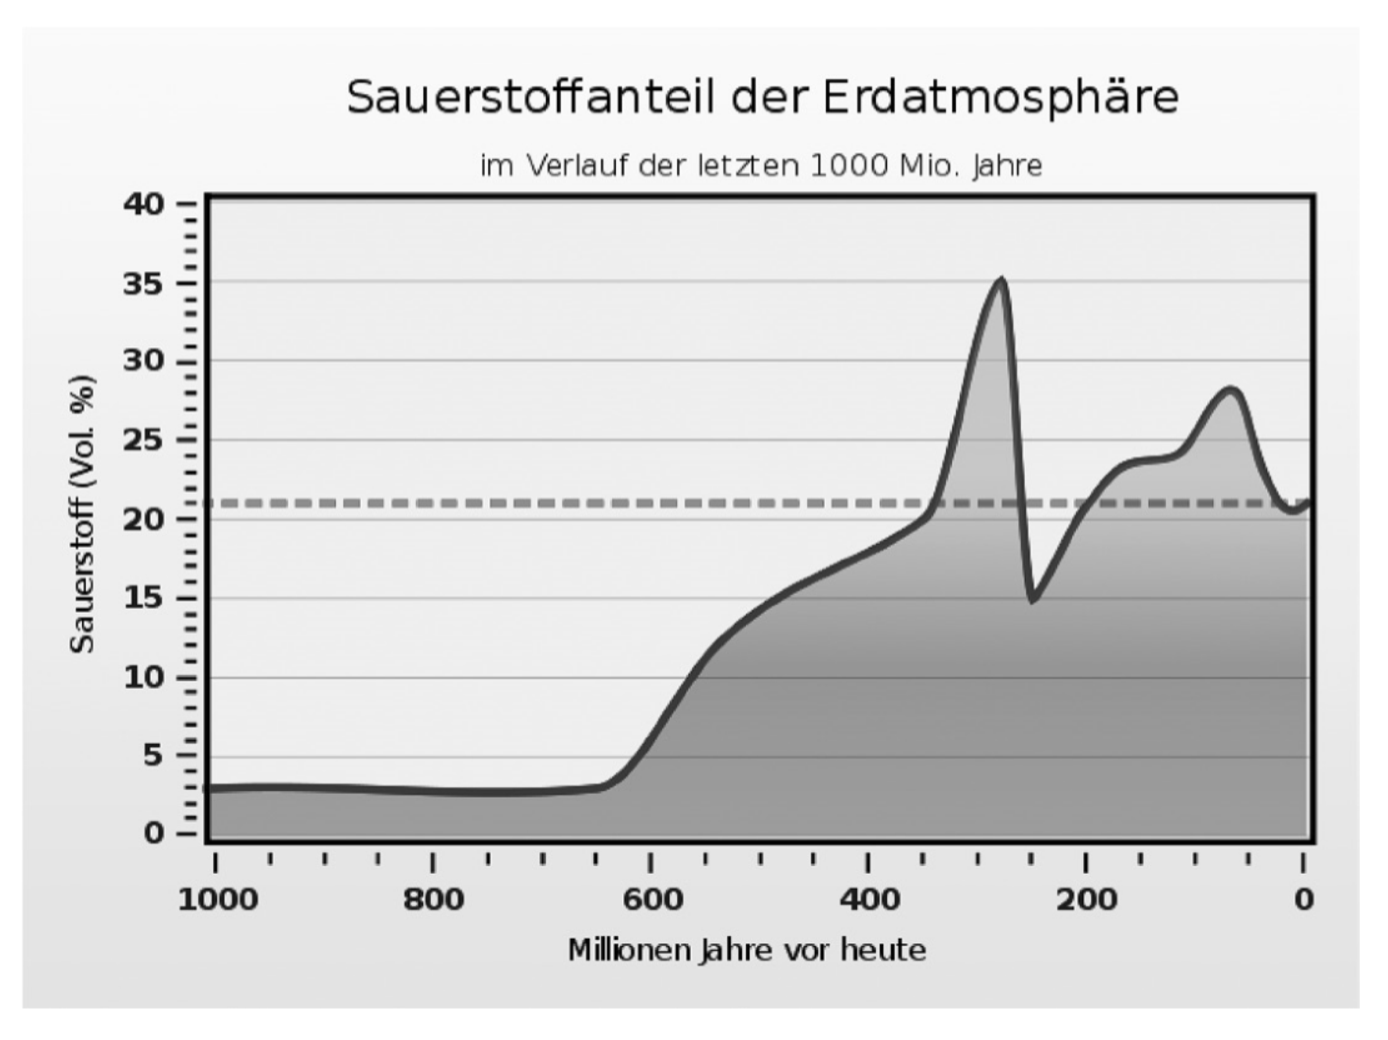
\includegraphics{../Bilder/Bild42-2.eps}}
	\end{center}
	\begin{footnotesize}\begin{singlespace}\textit{Abb. 2: Darstellung des Sauerstoffgehaltes in der Atmosphäre im Verlauf der letzten Milliarden Jahre}\end{singlespace}\end{footnotesize}
	
\subsection{Aufgabenstellung:}
\begin{enumerate}
	\item Stelle ein exponentielles Wachstumsgesetz der Form $K(t)=K_0\cdot a^t$ auf, das die CO$_2$-Konzentration $K$ in Abhängigkeit von der Zeit $t$ in der Atmosphäre wiedergibt! Dabei gibt $t$ die seit 1950 vergangene Zeit in Jahren an; $K$ wird in ppm und $t$ in Jahren gemessen. Lies zur Bestimmung der Parameter $K_0$ und $a$ die auf Zehner gerundeten Konzentrationen der Jahre 1950 und 1980 (Endpunkt der Aufzeichnungen) aus der entsprechenden Grafik ab!
	
	Kreuze die beiden zutreffenden Aussagen an!
	
	\multiplechoice[5]{  %Anzahl der Antwortmoeglichkeiten, Standard: 5
					L1={Die CO$_2$-Konzentration steigt im beobachteten Zeitraum um ca. $0,4\,\%$ pro Jahr.},   %1. Antwortmoeglichkeit 
					L2={Die CO$_2$-Konzentration steigt im beobachteten Zeitraum um ca. 4 ppm pro Jahr.},   %2. Antwortmoeglichkeit
					L3={Wäre der Wert von $a$ (bei gleichbleibendem Wert von $K_0$) doppelt so groß, so wäre auch der jährliche prozentuelle Zuwachs doppelt so groß.},   %3. Antwortmoeglichkeit
					L4={Für das Jahr 2010 werden nach diesem Wachstumsgesetz ca. 395 ppm prognostiziert.},   %4. Antwortmoeglichkeit
					L5={Wäre der Wert von $K_0$ (bei gleichbleibendem Wert von $a$) doppelt so groß, so wäre auch die Verdopplungszeit doppelt so groß.},	 %5. Antwortmoeglichkeit
					L6={},	 %6. Antwortmoeglichkeit
					L7={},	 %7. Antwortmoeglichkeit
					L8={},	 %8. Antwortmoeglichkeit
					L9={},	 %9. Antwortmoeglichkeit
					%% LOESUNG: %%
					A1=1,  % 1. Antwort
					A2=4,	 % 2. Antwort
					A3=0,  % 3. Antwort
					A4=0,  % 4. Antwort
					A5=0,  % 5. Antwort
					}
	
		\item Von 1800 bis 1900 ist der CO$_2$-Gehalt der Atmosphäre annähernd linear gewachsen. Stelle einen funktionalen Zusammenhang $K(t)$ zwischen der CO$_2$-Konzentration $K$ (gemessen in ppm) und der Zeit $t$ (gemessen in Jahren) auf! Dabei gibt $t$ die seit 1800 vergangene Zeit in Jahren an. Lese die auf Zehner gerundeten notwendigen Daten aus der Grafik ab!  Weise nach, dass der im Jahr 2010 tatsächlich gemessene CO$_2$-Wert von 390 ppm nicht das Ergebnis einer linearen Zunahme der historischen CO$_2$-Werte sein kann!

	
		\item Der Sauerstoffgehalt der Atmosphäre ist in den letzten 1 000 Mio. Jahren massiven Schwankungen unterworfen gewesen. Von 300 Mio. Jahren vor unserer Zeit bis 250 Mio. Jahren vor unserer Zeit hat der Sauerstoffgehalt annähernd linear abgenommen (siehe Abb. 2).
		
		\fbox{A} Berechne den Ausdruck $\frac{35-15}{300-250}$ und deute das Ergebnis in diesem Zusammenhang!
		
		Kreuze die zutreffende(n) Aussage(n) an!
		
		\multiplechoice[5]{  %Anzahl der Antwortmoeglichkeiten, Standard: 5
						L1={In den letzten 1 000 Mio. Jahren war der Sauerstoffgehalt der Atmosphäre meistens niedriger als heute.},   %1. Antwortmoeglichkeit 
						L2={Vor 250 Mio. Jahren war der Sauerstoffgehalt am absolut geringsten.},   %2. Antwortmoeglichkeit
						L3={In den letzten 600 Mio. Jahren ist der Sauerstoffgehalt der Atmosphäre nie unter 5 Volumsprozent gefallen.},   %3. Antwortmoeglichkeit
						L4={Vor 200 Mio. Jahren war der Sauerstoffgehalt der Atmosphäre etwa so groß wie heute.},   %4. Antwortmoeglichkeit
						L5={Vor 900 Mio. Jahren lag der Sauerstoffgehalt der Atmosphäre um 15 Volumsprozent niedriger als heute.},	 %5. Antwortmoeglichkeit
						L6={},	 %6. Antwortmoeglichkeit
						L7={},	 %7. Antwortmoeglichkeit
						L8={},	 %8. Antwortmoeglichkeit
						L9={},	 %9. Antwortmoeglichkeit
						%% LOESUNG: %%
						A1=1,  % 1. Antwort
						A2=3,	 % 2. Antwort
						A3=4,  % 3. Antwort
						A4=0,  % 4. Antwort
						A5=0,  % 5. Antwort
						}
						
		\item Die Funktionsgleichung $y(t)=0,000128\cdot t^3+0,01344\cdot t²+0,2304\cdot t$ beschreibt die absoluten Schwankungen des Sauerstoffgehalts bezogen auf den heutigen Wert $y(0)=0$ in der Atmosphäre in den letzten 100 Mio. Jahren. Dabei wird $t$ in Mio. Jahren und $y$ in Volumsprozent angegeben. Berechne, wann in diesem Zeitraum ein lokales Maximum des Sauerstoffgehaltes aufgetreten ist! Weise nach, dass es sich wirklich um ein lokales Maximum handelt!
						\end{enumerate}\leer
				
\antwort{
\begin{enumerate}
	\item \subsection{Lösungserwartung:} 
	
		$K(t)=310\cdot\left(\sqrt[30]{\frac{350}{310}}\right)^t$
		
		oder:
		
		$K(t)=310\cdot 1,004^t$
	 	
	\subsection{Lösungsschlüssel:}
	\begin{itemize}
		\item  Ein Punkt für das korrekte Aufstellen von $K(t)$. Toleranzintervall für $a$: $[1,004;1,0041]$.
		\item  Multiple-Choice-Aufgabe: Ein Punkt ist genau dann zu geben, wenn ausschließlich die beiden laut Lösungserwartung richtigen Antwortmöglichkeiten angekreuzt sind.

	\end{itemize}
	
	\item \subsection{Lösungserwartung:}
			
		1800: 280\,ppm
		
		1900: 300\,ppm\leer
		
		$K(t)=k\cdot t+d$
		
		$300=k\cdot 100+280 \Rightarrow k=0,2$\leer
		
		$K(t)=0,2\cdot t+280$\leer
		
		$K(210)=322$\,ppm $\neq$ 390\,ppm
		
	\subsection{Lösungsschlüssel:}
	
\begin{itemize}
	\item  Ein Punkt für das korrekte Aufstellen von $K(t)$.
	\item  Ein Punkt für einen korrekten Nachweis. 
\end{itemize}

\item \subsection{Lösungserwartung:}
			Der Ausdruck besagt, dass im angegebenen Zeitraum der Sauerstoffgehalt um 0,4 Prozentpunkte pro 1 Million Jahre abnimmt.
		
	\subsection{Lösungsschlüssel:}
	
\begin{itemize}
	\item  Ein Ausgleichspunkt für die richtige Lösung und eine (sinngemäß) korrekte Deutung.
	\item  Multiple-Choice-Aufgabe: Ein Punkt ist genau dann zu geben, wenn ausschließlich alle laut Lösungserwartung richtigen Antwortmöglichkeiten angekreuzt sind. 
\end{itemize}

\item \subsection{Lösungserwartung:}
			$y'(t)=0,000384t²+0,02688t+0,2304$
			
			$y''(t)=0,000768t+0,02688$\leer
			
			$y'(t)=0 \Rightarrow t_1=-60, t_2=-10$
			
			$y''(-10)>0 \Rightarrow$ Minimum
			
			$y''(-60)<0 \Rightarrow$ Maxmimum bei -60 Mio. Jahren
			
			Vor 60 Millionen Jahren ist ein lokales Maximum des Sauerstoffgehaltes aufgetreten.\leer
			
			Alternative Möglichkeiten des Maximumnachweises:\leer
			
			Es wird nachgewiesen, dass die Ableitungsfunktion $y'(x)$ links vom lokalen Maximum positiv und dass sie rechts vom lokalen Maximum negativ ist.\leer
			
			oder:\leer
			
			Es wird nachgewiesen, dass gilt: $y(-60-a)<y(-60)$ und $y(-60+a)<y(-60)$ für eine reelle Zahl $a$.\leer
			
			oder:\leer
		
		Es wird argumentiert, dass bei einer Polynomfunktion dritten Grades mit positiven Koeffizienten die kleinere Nullstelle der ersten Ableitung eine lokale Maximumstelle ist.\leer
		
		oder:\leer
		
		Weil $y(-60)>y(-10)$ und $y$ ein Polynom 3. Grades ist, muss das lokale Maximum bei $t=-60$ liegen.\leer
		
		oder:\leer
		
		Es gilt: $$\lim_{t \to -\infty} y(t)=-\infty$$ $$\lim_{t \to \infty} y(t)=\infty$$ $$y(-60)\approx 6,91$$$$ y(-10)\approx -1,09$$.
		
		Deshalb ist bei $t=-60$ ein lokales Maximum des Sauerstoffgehaltes.
	\subsection{Lösungsschlüssel:}
	
\begin{itemize}
	\item   Ein Punkt für die korrekte Berechnung der Jahreszahl (es genügt, als Lösung -60 Mio. Jahre anzugeben).
	\item   Ein Punkt für einen (sinngemäß) korrekten Nachweis.
\end{itemize}
\end{enumerate}}
		\end{langesbeispiel}